
\chapter{Estado del arte y fundamentos teóricos}\label{estadoArte}

En este capítulo analizaré el estado actual del tema a tratar, junto con una pequeña revisión bibliográfica y algunos conceptos teóricos necesarios. Y profundizaré un poco más en las representaciones lineales comentadas en el Capítulo \ref{introduccion}, así como los distintos paquetes software existentes y sus limitaciones. 

\section{Revisión bibliográfica} \label{revision_bib}
Para el estudio de los trabajos relacionados y búsqueda de bibliografía se han consultado fuentes como IEEE Xplore, ACS Publications, o Journal of Chemical Information and Computer Sciences entre otras. En la Figura \ref{fig:revisionBibliografica} se exponen los resultados de un breve estudio bibliográfico sobre la literatura existente de los temas del proyecto. Todo comienza en 1988 con la publicación de David Weininger \cite{weininger_smiles_1988}, presentando SMILES como un nuevo formato de representación lineal, a partir de ahí y hasta día de hoy, fueron aumentando las publicaciones alrededor de SMILES. Sin embargo, vemos que apenas existe literatura para temas más específicos dentro de este área, como la canonización de las cadenas SMILES, o la organometálica. Además, si nos paramos a revisar las publicaciones existentes vemos que apenas ninguna coincide con el reto de este proyecto, y mucho menos hacen alguna propuesta de cómo darle solución. Los datos de las publicaciones se han recopilado a través de \textit{Scopus}\footnote{\url{https://www.elsevier.com/es-es/solutions/scopus}}\footnotecomma\footnote{\url{https://biblioteca.ugr.es/investigacion/herramientas-apoyo/evaluacion-publicaciones/scopus}} con las siguientes consultas, donde CHEM y COMP hacen referencia a chemistry y computer science respectivamente: 
\begin{itemize}
    \item {\footnotesize \textit{(SUBJAREA(CHEM) AND TITLE-ABS-KEY(smiles))}} 
    \item {\footnotesize \textit{((SUBJAREA(CHEM) OR SUBJAREA(COMP)) AND TITLE-ABS-KEY(smiles AND canonical))}}
    \item {\footnotesize \textit{(SUBJAREA(CHEM) AND TITLE-ABS-KEY(smiles AND organometallic))}}
\end{itemize}

\begin{figure}[h!]
        \centering
        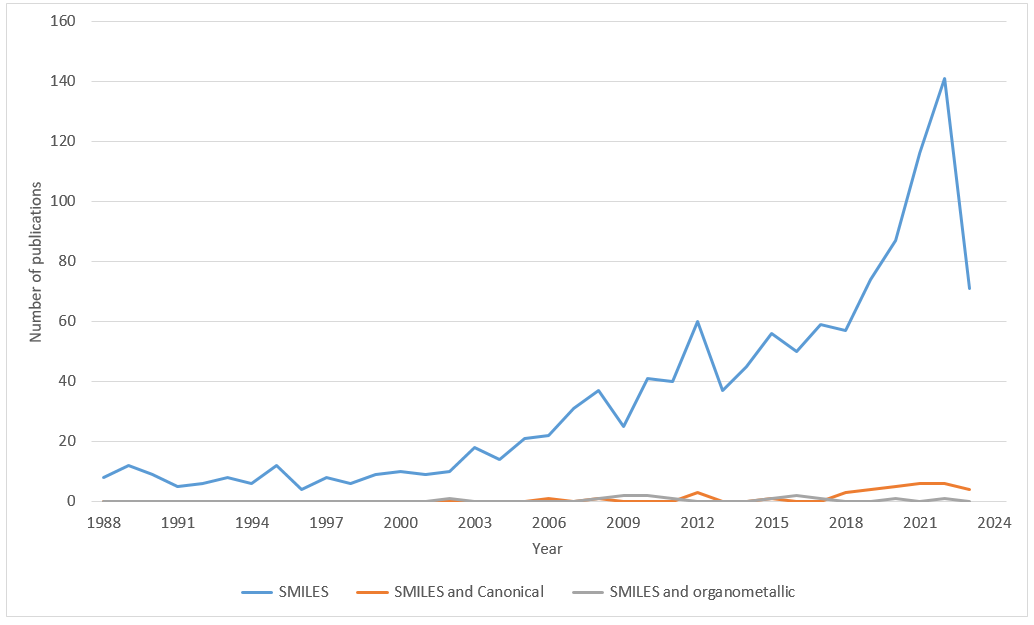
\includegraphics[scale=0.5]{imagenes/estado_arte/revisionBibliografica.png}
        \caption{Comparativa del número de artículos publicados por año según las palabras clave de la búsqueda. Imagen de elaboración propia. Datos extraídos de \emph{Scopus}.}
        \label{fig:revisionBibliografica}
    \end{figure}


\section{Fundamentos teóricos}

\subsection{Moléculas y sus representaciones}
representacion de moléculas (formula estructural conection tables, tipos de ficheros (.smi, .sdf, etc) representacion lineal y mas cosas),

\subsection{Representaciones lineales}
Hablar mas extendido de SMILES, SELFIES, e INCHI;

\subsection{Organometálica}
Cualquier concepto de quimica que me haga falta para entender el trabajo, o que haya tenido que aprender yo durante el mismo.
hablar de la regla de los 18 electrones y compuestos de coordinacion vs organometalicos
(mirar mashup)
hablar de los electrones y bonds delocalized

\section{Herramientas o toolkits} \label{toolkits}

Existe una gran variedad de herramientas a la hora de trabajar dentro de la química computacional, tanto open-source como aplicaciones propietarias para las que son necesarias pagar una licencia de uso. La química computacional según comenté en el capítulo \ref{introduccion}, se aplica en muchos ámbitos de la ciencia. Como tal, hay herramientas con propósitos muy distintos \cite{toolkits_recap}: 
\begin{itemize}
    \item Extensiones de navegador que mejoran el acceso a la información de las bases de datos \cite{safari_extensions}.
    \item Cálculos de propiedades fisicoquímicas (casi cualquier herramienta lo permite)
    \item Cribado virtual de moléculas como \textit{ChemAxon}, \textit{MOE}, \textit{LigandScout} o \textit{Forge}.
    \item Modelado y bocetado de moléculas como \textit{Marvin}, \textit{ChemDraw} o \textit{ChemDoodle}.
    \item Hojas de cálculo con análisis de datos químicos como \textit{Vortex}.
    \item Toolkits de propósito general con diversas funcionalidades básicas como \textit{OpenBabel} o \textit{RDKit}.
\end{itemize}
Las herramientas más complejas o relacionadas de alguna manera con la medicina suelen ser de pago. Para los objetivos de este proyecto se han tenido en cuenta los toolkits de propósito general mencionados anteriormente que son capaces de trabajar con SMILES.

\subsection{OpenBabel y RDKit}

Openbabel y RDKit son bastante parecidos en cuanto a sus funcionalidades, ambos permiten la manipulación de estructuras químicas, cálculos de propiedades moleculares, análisis de similitudes entre moléculas, generación de representaciones 2D y conversión entre distintos tipos de ficheros. Para elegir entre una de estas 2 herramientas, se han hecho pruebas iniciales en un notebook de Google Colab \cite{google_colab} (disponible con un enlace de acceso en GitHub)


RDKit por su parte, consigue representaciones 2D parecidas o mejores que las de OpenBabel para moléculas pequeñas y cuenta con mayores opciones de personalización del dibujo resultado \cite{rdkit_cookbook} haciéndolo más visual. Además, es más preciso a la hora de representar la estereoquímica, algo en lo que OpenBabel es bastante pobre. Vemos en la Figura \ref{fig:ejemplo_rdkit_vs_babel} un ejemplo con ambos paquetes software. Sin embargo, si se le exige un poco más a RDKit pidiéndole moléculas complejas no funciona del todo bien. Concretamente, cuando introducimos moléculas de organometálica no las lee correctamente aun siendo químicamente válidas. RDKit lleva a cabo un proceso de 'saneamiento' (\textit{sanitization}) \cite{rdkit_docbook} por el que, además de calcular algunas propiedades útiles (pertenencia de los átomos a anillos o hibridaciones), comprueba que la molécula de entrada es 'razonable'. Para RDKit, serán razonables las moléculas que cumplan la regla del octeto\footnote{\url{https://acortar.link/regla_octeto}} y puedan representarse mediante las estructuras de Lewis de manera completa. Como hemos visto anteriormente, los compuestos de coordinación se rigen por otro tipo de sistema de valencia, y RDKit no es capaz de trabajar con esta clase de moléculas. De hecho, del set de moléculas del que dispongo para el proyecto, no es capaz de leer ningún código SMILES de los que fueron extraídos de SciFinder. Los SMILES de SigmaAldrich si los puede usar, pero más adelante en esta misma Sección se explicará por qué estos no nos sirven.

\begin{figure}[h!]
\centering
\begin{subfigure}{.5\textwidth}
  \centering
  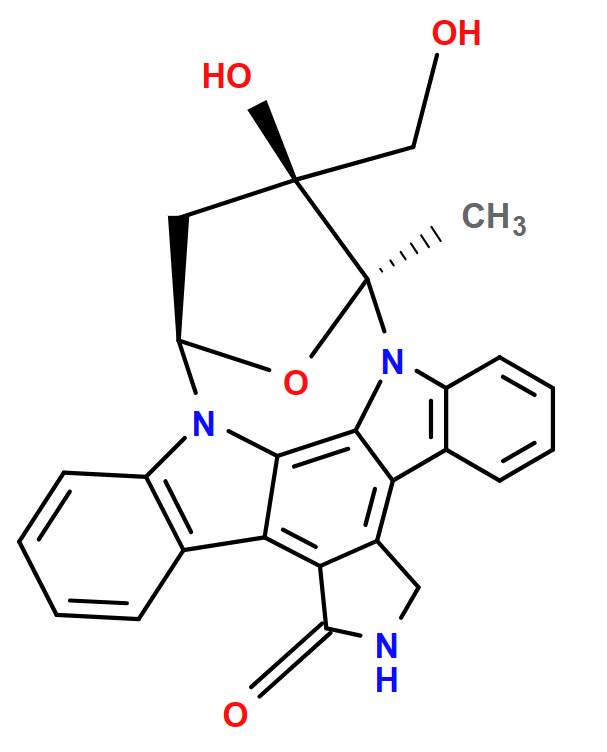
\includegraphics[width=.7\linewidth]{imagenes/estado_arte/Lestaurtinib_openbabel.png}
  \caption{OpenBabel}
  \label{fig:sub1}
\end{subfigure}%
\begin{subfigure}{.5\textwidth}
  \centering
  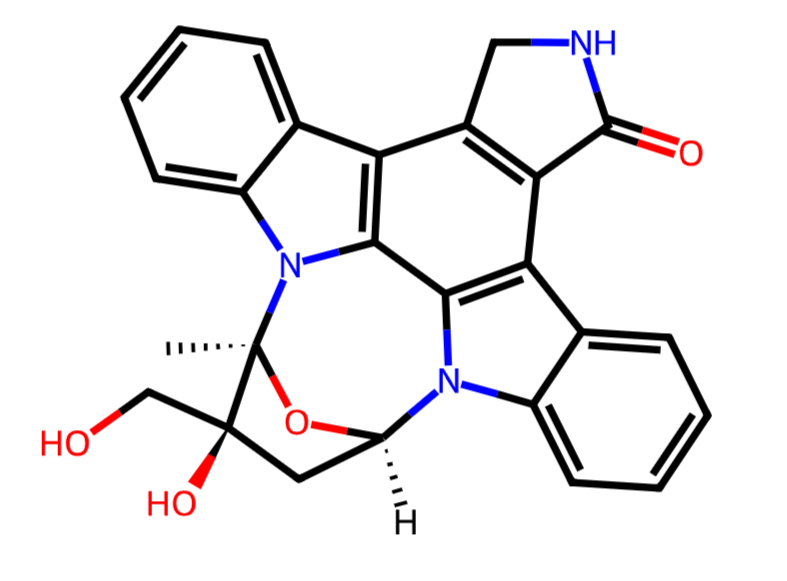
\includegraphics[width=.9\linewidth]{imagenes/estado_arte/Lestaurtinib_rdkit.png}
  \caption{RDKit}
  \label{fig:sub2}
\end{subfigure}
\caption{Representaciones 2D para el \emph{Lestaurtinib}, medicamento en estudio para el tratamiento de las leucemias agudas y algunos otros tipos de cáncer. \textbf{(a)} ha sido generado con OpenBabel; y \textbf{(b)} ha sido generado con RDKit.}
\label{fig:ejemplo_rdkit_vs_babel}
\end{figure}



OpenBabel por otro lado, ofrece más libertad en este sentido siendo capaz de leer todos los SMILES del set del que partimos. Pero en general, algo que hacen mal ambos paquetes es dibujar. Para moléculas convencionales, moléculas orgánicas o inorgánicas sencillas funciona bien, pero las organometálicas les supone un reto, y dada la escasa literatura en el tema (ver Sección \ref{revision_bib}), no dispongo de muchas referencias de las que partir.


En cuanto a los datos de partida contamos con 2 versiones de SMILES, los provenientes de SigmaAldrich y los de SciFinder. Siguiendo la comparación de la Sección \ref{motivacion} ambos SMILES son notablemente distintos, de hecho no se podrían considerar ni siquiera sinónimos ya que al de SigmaAldrich le faltan enlaces, y no llegan a codificar la misma molécula. Tanto es así que las cadenas SMILES que contienen desconexiones (representadas por el punto '.') no nos son para nada útiles. Al fragmentar la molécula estamos perdiendo los enlaces entre los átomos, una información muy valiosa para la mayoría de operaciones. Como se dijo antes, una molécula se suele almacenar principalmente identificando sus átomos y los enlaces entre sus átomos. Podríamos decir que se está perdiendo casi la mitad de la información acerca de la molécula, y dado que uno mismo no puede inventarse los enlaces, no es un buen SMILES para nuestros objetivos, ni para la canonización ni para el dibujado. En la Figura \ref{fig:dotted_smiles_vs_complete} vemos la diferencia entre la representación de un SMILES inconexo frente a uno con buena conectividad.


\begin{figure}[h!]
\centering
\begin{subfigure}{.5\textwidth}
  \centering
  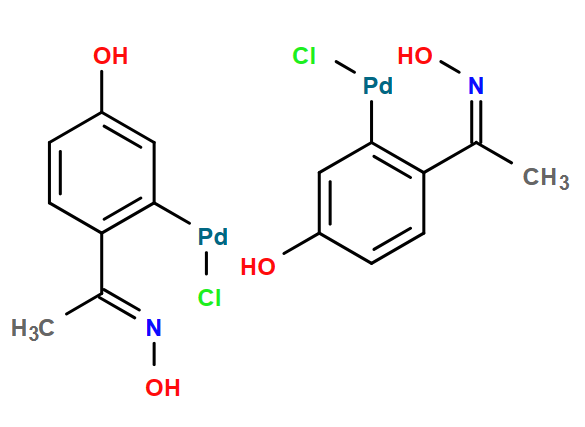
\includegraphics[width=.9\linewidth, frame]{imagenes/estado_arte/dotted_SA.png}
  \caption{}
  \label{fig:sub1}
\end{subfigure}%
\begin{subfigure}{.5\textwidth}
  \centering
  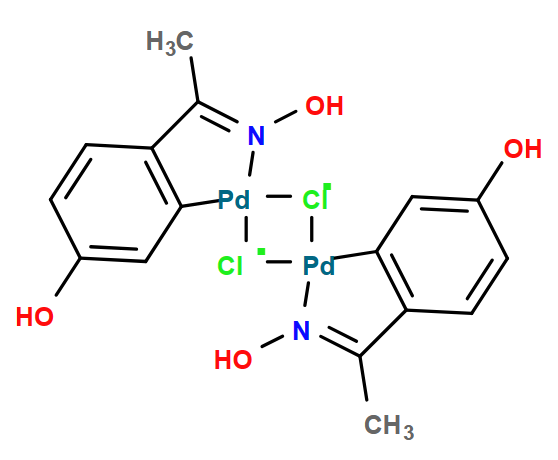
\includegraphics[width=.8\linewidth, frame]{imagenes/estado_arte/not_dotted_SF.png}
  \caption{}
  \label{fig:sub2}
\end{subfigure}
\caption{Representaciones 2D generadas con OpenBabel para el \emph{'Nájera Catalyst II'}. \textbf{(a)} SMILES con desconexiones extraído de SigmaAldrich; y \textbf{(b)} SMILES conectado extraído de SciFinder.}
\label{fig:dotted_smiles_vs_complete}
\end{figure}


\subsection{Herramientas de bocetado}
Simplemente para mencionarlas, herramientas tipo ChemDraw \cite{chemdraw_page} son las que los químicos e investigadores utilizan para dibujar manualmente las moléculas que luego añaden a sus publicaciones. Son este tipo de dibujos también los que probablemente podemos ver en algunas bases de datos como SigmaAldrich. En la Figura \ref{fig:chemdraw} se muestra su interfaz y algunas moléculas bocetadas.

\begin{figure}[h!]
    \centering
    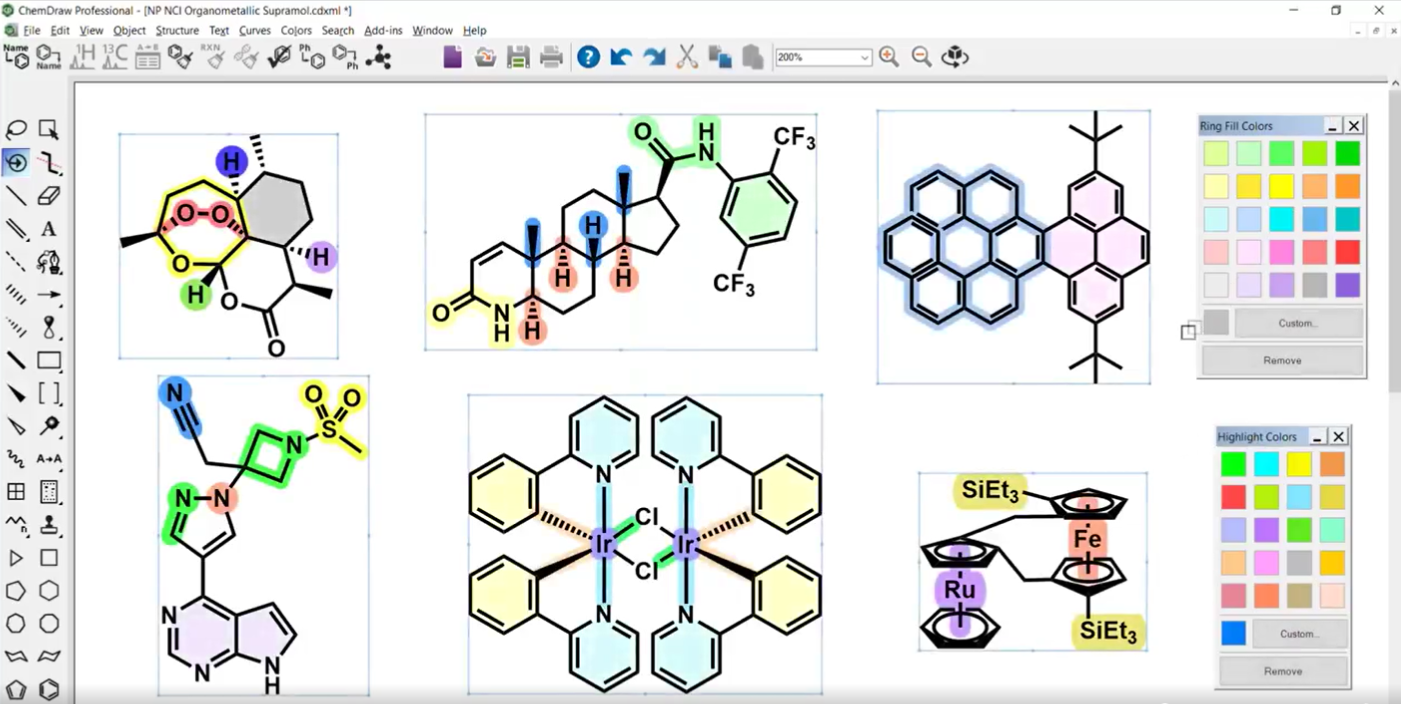
\includegraphics[scale=0.34]{imagenes/estado_arte/chemdraw.png}
    \caption{Interfaz de ChemDraw con algunas moléculas de prueba bocetadas. Imagen extraída de su página oficial \cite{chemdraw_page}}
    \label{fig:chemdraw}
\end{figure}

\subsection{Nomenclatura canónica}
Como ya se ha visto, InChI proporciona una representación canónica para las moléculas, lo que permite una vinculación directa y unívoca entre las bases de datos. SMILES por otro lado complica este proceso. SMILES fue desarrollado en su momento como un software propietario por Daylight Chemical Information Systems (Daylight) \cite{daylight}, y desde su introducción a finales de los 80 se ha extendido como una norma de facto para representar estructuras moleculares. En base a esto y con el tiempo, se han escrito en varios lenguajes de programación muchos paquetes de software independientes que trabajan con SMILES a su manera\cite{opensmiles}.

Bien es cierto que hay cada vez más propuestas de cómo alcanzar una nomenclatura única \cite{weininger_smiles_1989, inchi1, nextmove_software_facto_nodate, baoilleach_we_nodate, universal_smiles} y ya existen algunas reglas definidas para la química orgánica a la hora de establecer prioridades entre los átomos y ordenar la molécula. Véase por ejemplo las \emph{'Reglas de Cahn-Ingold-Prelog'} aplicadas a enantiómeros \cite{cahn_specification_1966, prelog_basic_1982, NOMENCLATURA_R_S} para definir ordenes levógiros o dextrógiros (no abordaremos esto, excede el alcance del proyecto). Pero trasladar estas reglas a compuestos organometálicos es complicado, además de haber multitud de excepciones, en la mayoría de casos un mismo fragmento está enlazado por varios sitios al metal y hay que definir el átomo inicial por el que empezar a recorrer la molécula. Al final, cada paquete software implementa esta decisión de una manera diferente usando un algoritmo propio, obteniendo así lo que cada uno de ellos nombra como 'canonical SMILES', pero siguen siendo distintos entre ellos, por lo que no es canónico.

\subsection{Conclusiones}
Dicho todo lo anterior, durante las pruebas realizadas se ha podido comprobar y extraer las siguientes conclusiones:

\begin{itemize}
    \item Al representar la misma molécula con herramientas distintas, lo normal es que generen dibujos diferentes, que no tiene por qué estar mal, pero por lo general uno será mejor o más correcto que el otro.
    \item Para una misma molécula, es probable que cada base de datos muestre una cadena SMILES diferente y una representación 2D distinta. De hecho, la imagen puede ni siquiera concordar con el SMILES que ofrecen, apareciendo en multitud de casos por ejemplo, un SMILES desconectado y una imagen con la molécula al completo (lo más seguro es que estén hechos a mano)
    \item Vistos los resultados de los SMILES de SigmaAldrich, para el resto del proyecto se asumirá que se trabaja con los SMILES de SciFinder, ya que dotan de mejor conectividad. 
    \item Debido a lo anterior, y como RDKit no soporta los datos de entrada, se utilizará la librería de OpenBabel para el proyecto.
    \item Hay diversos tipos de compuestos que no se describen bien mediante la representación de su grafo molecular, como los compuestos de coordinación. Su sistema de enlaces no se ajusta a la teoría de los enlaces de valencia, por lo que es complejo describir sus enlaces mediante relaciones 1 a 1 entre los átomos \cite{david_molecular_2020}.
    \item Moléculas complejas con multitud de ciclos o muchos enlaces al mismo átomo (generalmente un metal), Openbabel genera unas representaciones 2D muy agrupadas, con los enlaces superpuestos y partes del dibujo unas encima de las otras, dificultando su entendimiento.
    \item Hasta ahora, no hay ningún sistema de canonizado que trabaje de manera eficiente con moléculas organometálicas.
    
\end{itemize}


Teniendo esto en cuenta y lo mencionado en la Sección \ref{motivacion}, en las siguientes secciones se dará pie a una posible implementación de una nomenclatura canónica para moléculas organometálicas y la mejora del dibujado de las mismas con OpenBabel.





